%=======================================================================
%  GalaxyCBM-SR
%  Glass-box galaxy morphology: symbolic concept bottlenecks
%
%  JOURNAL-NEUTRAL MANUSCRIPT FORMAT
%  Single-column, 11pt, generous margins, 1.5 line spacing.
%  Most journals (MNRAS, A&A, ApJ, MLST, Sci Rep, A&C) accept this for
%  initial submission under "your paper, your way" policies. Convert to a
%  house class only if the journal requests it after review.
%
%  Compile:  pdflatex main && pdflatex main && pdflatex main
%  Figures expected in paper/figures/ (regenerate with `make eval`)
%=======================================================================
\documentclass[11pt]{article}

\usepackage[a4paper,margin=2.5cm]{geometry}
\usepackage[T1]{fontenc}
\usepackage[utf8]{inputenc}
\usepackage{graphicx}
\usepackage{amsmath,amssymb}
\usepackage{booktabs}
\usepackage{multirow}
\usepackage{xcolor}
\usepackage{siunitx}
\usepackage{float}
\usepackage[ruled,vlined,linesnumbered]{algorithm2e}
\usepackage[round,authoryear]{natbib}
\usepackage{setspace}
\usepackage{caption}
\providecommand{\doi}[1]{doi:\href{https://doi.org/#1}{#1}}
\usepackage[colorlinks=true,citecolor=blue,linkcolor=blue,urlcolor=blue]{hyperref}

\onehalfspacing

\captionsetup{font=small,labelfont=bf}
\setlength{\parskip}{0pt}

\newcommand{\kappastat}{\ensuremath{\kappa}}
\newcommand{\code}[1]{\texttt{\small #1}}
\sisetup{detect-weight=true,detect-family=true}

% Standard AAS/ADS journal abbreviations, used in the reference list.
\providecommand{\aap}{A\&A}
\providecommand{\aj}{AJ}
\providecommand{\apj}{ApJ}
\providecommand{\apjl}{ApJL}
\providecommand{\apjs}{ApJS}
\providecommand{\araa}{ARA\&A}
\providecommand{\mnras}{MNRAS}
\providecommand{\pasp}{PASP}
\providecommand{\nat}{Nature}

\begin{document}

%=======================================================================
\title{\bfseries Interpretable Machine Learning for Galaxy Morphology:
A Calibrated Symbolic Concept Bottleneck, and Why Its Explanations Do Not
Transfer Across Surveys}

\author{
  Ram Chand\thanks{Correspondence: \texttt{ram.chand2k11@yahoo.com}}\\[2pt]
  \normalsize Department of Natural Sciences,\\
  \normalsize The Begum Nusrat Bhutto Women University, Sukkur, Sindh, Pakistan
}

\date{\today}

\maketitle

\begin{abstract}
Deep networks classify galaxy morphology at survey scale but expose no
auditable reasoning, and post-hoc attributions explain a surrogate rather than
the deployed decision. We present the first Concept Bottleneck Model for
galaxy morphology: a \textsc{Zoobot} ConvNeXt predicts seventeen physically
named concepts---ten Galaxy Zoo tasks and seven \textsc{statmorph}
statistics---and a symbolic-regression head of 153 operator nodes, printed in
full, maps them to a Hubble type under split-conformal uncertainty. On
$40\,498$ Galaxy Zoo Evo galaxies we quantify what interpretability costs
rather than claiming it is free: an unconstrained ConvNeXt reaches
$\kappa=0.601$ against the symbolic head's $0.571$, so the bottleneck gives up
$0.030$, while symbolic, dense-linear and boosted-tree heads over the same
concepts agree to within $0.002$. The cost is therefore attributable to the
concept layer, not to the symbolic form, which is obtained at no further
penalty and replaces $1.5\times10^{7}$ parameters. Two findings qualify this.
Conformal coverage is marginally exact ($88.9\%$ against a $90\%$ target) but
conditionally severe: per-class coverage spans $0.98$ for ellipticals to
$0.08$ for the rarest spiral, so the guarantee is met by over-covering the
dominant class---a failure mode that directly threatens rare-object science.
Applying the frozen pipeline to $161\,395$ Euclid Q1 galaxies preserves
accuracy while a symbolic refit recovers only $42\%$ of the reference rules'
concept usage. Accuracy transfer and interpretation transfer are distinct
properties, and an accuracy-only audit certifies a pipeline whose explanations
have silently changed. Code, seeds and a reproducible benchmark for concept
fidelity, conditional coverage and rule stability are released.
\end{abstract}

\vspace{4pt}
\noindent\textbf{Keywords:} galaxies: structure -- methods: data analysis -- techniques: image processing
-- machine learning -- deep learning -- interpretable machine learning --
symbolic regression -- conformal prediction


%=======================================================================
\section{Introduction}
\label{sec:intro}

Galaxy morphology encodes assembly history. Mergers, secular disc growth,
bar-driven inflows and quenching each leave structural signatures, and the
correlation of those signatures with mass, environment and star-formation rate
underpins much of our picture of galaxy evolution
\citep{hubble1926,conselice2014}. Surveys now deliver morphological data at a
volume that forecloses visual classification: Galaxy Zoo has aggregated
$\sim\!10^{8}$ volunteer classifications, and Euclid, LSST and Roman will
image billions of resolved sources.

Automated classifiers meet this volume, but the dominant approach---end-to-end
convolutional networks trained directly to a morphological
target~\citep{dieleman2015,dominguez2018,walmsley2022}---produces decisions in
a representation with no physical referent. When such a model assigns a galaxy
to Sb, nothing in its output identifies which structural property drove the
assignment. The standard remedy, post-hoc attribution via SHAP or saliency
maps~\citep{lundberg2017,smilkov2017}, fits a second model to approximate the
first; \citet{rudin2019} argues that this approximation routinely disagrees
with the computation it purports to describe, and that in consequential
settings one should instead constrain the model to be interpretable by
construction.

Concept Bottleneck Models~\citep{koh2020} implement that constraint. Every
prediction is forced through an intermediate layer of individually supervised,
named concepts; the final classifier sees nothing else. The architecture
remains active in interpretable-ML research, with post-hoc
construction~\citep{yuksekgonul2023} and label-free concept
discovery~\citep{oikarinen2023} both directed at the same practical
obstacle: obtaining a concept vocabulary and the annotations to supervise it.
Galaxy morphology does not have that problem. The Galaxy Zoo decision tree
already enumerates a curated perceptual
vocabulary (bar strength, bulge prominence, spiral arm count and winding,
edge-on orientation, disturbance), and non-parametric morphology supplies a
quantitative one (concentration, asymmetry, smoothness, Gini, $M_{20}$,
Sérsic index, effective radius) with three decades of physical calibration
behind it~\citep{conselice2003,lotz2004,rodriguez2019}. These are the
quantities in which morphologists already reason. Despite this, no published
CBM exists for galaxy morphology.

This paper closes that gap and adds three components that we argue are
prerequisites for deploying an interpretable classifier on survey data.

\emph{A symbolic decision head.} We replace the CBM's usual dense linear
layer with compact analytic expressions discovered by symbolic
regression~\citep{cranmer2023}. The deployed classifier is then a table of
seven equations that a referee can read, not a weight matrix over concepts.
Symbolic regression has been applied to astronomical classification boundaries,
notably in star--galaxy--quasar
separation~\citep{deshpande2026,llorella2025}, where compact analytic
functions of photometric colours recover competitive accuracy. Here the
symbolic model operates one level higher: its inputs are not raw observables
but predicted physical concepts, and the expression it recovers constitutes
the classifier itself rather than a summary of one.

\emph{Calibrated set-valued prediction.} Interpretability does not confer
reliability: a legible rule can be confidently wrong. We wrap the symbolic
head in split-conformal prediction~\citep{vovk2005,angelopoulos2023}, which
converts point predictions into label sets whose marginal coverage is
guaranteed without assuming the underlying score is a calibrated probability.
We then measure \emph{conditional} coverage per class, and find that the
marginal guarantee is nearly vacuous for the rarest morphologies
(Section~\ref{sec:calibration}).

\emph{An interpretability audit under domain shift.} Instruments differ in
pixel scale, passband and point-spread function, and non-parametric morphology
statistics are known to respond to all three~\citep{ferrari2015}. We therefore
ask a question that accuracy-based robustness studies cannot answer: after
transfer to a new survey, does a symbolic refit recover the same rules? We
quantify this with a concept-usage Jaccard index between reference and refit
rule sets. On Euclid Q1 the answer is no, even though accuracy is preserved
(Section~\ref{sec:robustness}).

\paragraph{Contributions.}
\begin{enumerate}
\item The first Concept Bottleneck Model for galaxy morphology, jointly
supervised on Galaxy Zoo vote fractions and \textsc{statmorph} structural
statistics, with per-concept fidelity reported against explicit trivial
baselines (Table~\ref{tab:fidelity}).
\item A symbolic concept head---153 operator nodes across seven classes,
printed in full---together with a measurement of what it costs: the concept
bottleneck gives up $0.030$ in $\kappa$ against an unconstrained ConvNeXt,
while the symbolic head matches a dense linear head and gradient-boosted trees
over the same concepts to within $0.002$. Expressing the classifier
symbolically is therefore free; restricting it to named concepts is not
(Table~\ref{tab:baselines}).
\item Evidence that marginal conformal coverage is an inadequate reliability
statement under the class imbalance endemic to morphology catalogues, with
per-class coverage spanning an order of magnitude (Table~\ref{tab:coverage}).
\item A rule-stability metric and the finding that symbolic explanations do
not transfer across surveys even when accuracy does, establishing
interpretation transfer as a target for evaluation distinct from accuracy
transfer (Table~\ref{tab:robustness}).
\end{enumerate}

Code, configurations, random seeds, trained rules and every number quoted
below are released (Section~\ref{sec:availability}).

%=======================================================================
\section{Data}
\label{sec:data}

\subsection{Primary sample}

We use Galaxy Zoo Evo~\citep{walmsley2025gzevo}, restricted to the DESI Legacy
Imaging pool (\code{dataset\_name = gz\_desi}), which aggregates the GZD-5 and
GZD-8 campaigns~\citep{walmsley2022,walmsley2023desi}. We process six of the
thirty released training shards, $\sim\!1.3\times10^{5}$ raw rows, delivered
as $224\times224$ three-band cutouts at the DECaLS native pixel scale of
$0.262''$. This is a deliberate subsample: \citet{walmsley2024scaling} show
that morphology-model performance on Galaxy Zoo imagery continues to improve
with training-set size, so the absolute metrics reported here should be read
as a floor rather than a ceiling for the architecture.

\subsection{Structural concepts}

We compute concentration $C$, asymmetry $A$, smoothness $S$, the Gini
coefficient, $M_{20}$, Sérsic index $n$ and elliptical half-light radius
$r_{\rm eff}$ for every cutout with \textsc{statmorph}
v0.7.2~\citep{rodriguez2019}. Segmentation uses \code{photutils}
\code{detect\_sources} at a $2.5\sigma$ threshold above a background estimated
from the frame corners; because Galaxy Zoo cutouts are centred and tightly
cropped, a global median background is biased high by the source itself, and
the corner estimate removes that bias. The same estimate is subtracted before
the morphology call.

Failures are recorded rather than silently propagated. A per-object bitmask
flags \textsc{statmorph} internal warnings, non-convergent Sérsic fits, absent
segmentation, and a $\SI{60}{\second}$ per-object wall-clock timeout---a small
population of images drives the Sérsic optimiser into non-terminating
iteration. Of $265\,692$ processed objects, $127\,816$ ($48.1\%$) carry at
least one flag and are excluded before label construction. A downstream
assertion refuses to proceed if any concept is \code{NaN} without a
corresponding flag, so no silent failure can reach the model.

\subsection{Morphological labels}

Hubble types $\{$E, S0, Sa, Sb, Sc, Sd, Irr$\}$ are derived from GZD-5 vote
fractions through a compact traversal of the Galaxy Zoo decision tree:
smooth-or-featured $\rightarrow$ merger test $\rightarrow$ edge-on test
$\rightarrow$ spiral-arm test $\rightarrow$ winding $\times$ bulge size for
spiral subtype. At each node we take the plurality answer subject to a
clean-sample threshold of $0.5$; objects for which no answer clears threshold
are discarded as unclassified. This yields $40\,498$ labelled galaxies.

\subsection{Splits and leakage control}

We partition into train ($24\,299$), validation ($6\,075$), calibration
($4\,049$) and test ($6\,075$) subsets, stratified by Hubble type under a fixed
seed. Leakage is excluded on two axes: exact object-identifier collision, and
on-sky proximity, rejecting any cross-split pair separated by less than
$3''$ (\code{astropy} \code{SkyCoord} cross-match). The second test matters
because independent vote aggregation can produce distinct identifiers for the
same physical object.

The resulting class distribution is severely imbalanced
(Table~\ref{tab:balance}): ellipticals constitute $66.7\%$ of the sample while
Sa and Sd together account for $0.6\%$. This imbalance is intrinsic to
volunteer-classified magnitude-limited samples, not an artefact of our cuts,
and it governs the interpretation of every aggregate metric below.

\begin{table}[htbp]
\centering
\caption{Class balance by split. Sa and Sd are represented by tens of objects,
which bounds what any method can learn about them and drives the gap between
accuracy and macro-$F_1$ throughout.}
\label{tab:balance}
\begin{tabular}{lrrrr}
\toprule
Class & Train & Val. & Calib. & Test \\
\midrule
E   & 16207 & 4052 & 2701 & 4052 \\
S0  &  2570 &  642 &  428 &  643 \\
Sb  &  2543 &  636 &  424 &  636 \\
Sc  &  1451 &  363 &  242 &  362 \\
Irr &  1375 &  344 &  229 &  344 \\
Sd  &   104 &   26 &   17 &   26 \\
Sa  &    49 &   12 &    8 &   12 \\
\midrule
Total & 24299 & 6075 & 4049 & 6075 \\
\bottomrule
\end{tabular}
\end{table}

\subsection{Cross-survey sample}

Euclid Q1 morphology data~\citep{euclid2025morphology} provides $161\,395$
galaxies after applying the identical label derivation to Euclid's own vote
fractions. No Euclid object enters Stage-1 training, Stage-2 rule discovery or
Stage-3 calibration. An HST/JWST COSMOS-Web sample is queued for identical
treatment pending dataset access.

%=======================================================================
\section{Methods}
\label{sec:methods}

The pipeline comprises three stages, each frozen before the next is evaluated.
Algorithm~\ref{alg:pipeline} states the procedure in full; the subsections
below give the reasoning behind each design choice.

\begin{algorithm}[htbp]
\SetAlgoLined
\DontPrintSemicolon
\KwIn{Images $\{x_i\}$; concept targets $\{c_i\}$ from Galaxy Zoo votes and
\textsc{statmorph}; Hubble labels $\{y_i\}$; splits
$\mathcal{D}_{\rm tr},\mathcal{D}_{\rm val},\mathcal{D}_{\rm cal},
\mathcal{D}_{\rm te}$; miscoverage level $\alpha$}
\KwOut{Rule set $\{g_k\}_{k=1}^{K}$; conformal threshold $\hat q$}
\vspace{2pt}
\textbf{Stage 1 --- concept predictor}\;
Initialise backbone $f_\theta$ from \textsc{Zoobot} pretrained weights\;
Attach one linear head per concept: softmax for the $M$ categorical Galaxy
Zoo tasks, scalar for the $P$ continuous structural statistics\;
Minimise
$\mathcal{L} = \sum_{m=1}^{M}\lambda_m\,\mathrm{CE}(\hat c_m, c_m)
             + \sum_{p=1}^{P}\lambda_p\,\mathrm{SmoothL1}(\hat c_p, c_p)$
on $\mathcal{D}_{\rm tr}$, early-stopping on $\mathcal{D}_{\rm val}$\;
Missing categorical targets are masked via \code{ignore\_index}; missing
continuous targets are masked in the loss\;
Emit predicted concept vectors $\hat c_i$ for \emph{all} splits\;
\vspace{2pt}
\textbf{Stage 2 --- symbolic head} \tcp*{consumes $\hat c$, never $c$}
\For{each class $k \in \{1,\dots,K\}$}{
  Form binary target $z_i = \mathbb{1}[y_i = k]$ on $\mathcal{D}_{\rm tr}$\;
  Run symbolic regression on $(\hat c, z)$ under a complexity budget,
  obtaining a Pareto front $\mathcal{P}_k$ of (expression, complexity) pairs\;
  \For{each candidate $g \in \mathcal{P}_k$}{
    Score $g$ by $R$-fold stratified cross-validated accuracy on held-out
    folds of $\mathcal{D}_{\rm tr}$\;
  }
  $g_k \leftarrow$ candidate maximising CV accuracy, ties broken toward
  lower complexity\;
}
Predict $\hat y(\hat c) = \arg\max_k g_k(\hat c)$\;
\vspace{2pt}
\textbf{Stage 3 --- conformal calibration}\;
$s_i \leftarrow 1 - \mathrm{softmax}_k\!\left[g_k(\hat c_i)\right]_{y_i}$
for $i \in \mathcal{D}_{\rm cal}$ \tcp*{LAC score}
$\hat q \leftarrow \lceil (n_{\rm cal}+1)(1-\alpha)\rceil / n_{\rm cal}$
empirical quantile of $\{s_i\}$\;
$C(x) \leftarrow \{k : 1 - \mathrm{softmax}_k[g(\hat c)] \le \hat q\}$\;
\Return $\{g_k\},\ \hat q$\;
\caption{Symbolic concept-bottleneck classification with conformal
uncertainty.}
\label{alg:pipeline}
\end{algorithm}

\subsection{Stage 1: concept predictor}
\label{sec:stage1}

We fine-tune a \textsc{Zoobot} \code{convnext\_nano}
backbone~\citep{walmsley2023zoobot,liu2022convnext}, pretrained on Galaxy Zoo
imaging, attaching one linear head per concept: cross-entropy for the ten
categorical Galaxy Zoo tasks, smooth-$L_1$ for the seven continuous structural
statistics, summed with equal weight across provenance classes. Optimisation
uses AdamW at learning rate $3\times10^{-4}$, weight decay $10^{-4}$, mixed
precision, gradient clipping at $1.0$, and early stopping on validation loss
within a 40-epoch budget.

Concept fidelity is reported per concept against an explicit trivial baseline:
area under the ROC curve against $0.5$ for categorical concepts, and root-mean-square
error against the standard deviation of the training target for continuous
ones. A concept that fails to beat its baseline is reported as such rather
than aggregated away.

\subsection{Stage 2: symbolic decision head}
\label{sec:stage2}

The symbolic head consumes \emph{predicted} concepts $\hat c$, never ground
truth. This is the property that makes the pipeline interpretable end to end:
at inference no privileged information exists anywhere between pixels and
label, so the rule set is a complete description of the deployed decision.

For each Hubble class we fit one symbolic regression against the binary
one-vs-rest indicator, following the formulation used for symbolic
star--galaxy--quasar separation~\citep{deshpande2026}. We use
PySR~\citep{cranmer2023} with 100 iterations, a maximum expression size of 25
nodes, parsimony $3.2\times10^{-3}$, binary operators
$\{+,-,\times,\div\}$ and unary operators
$\{\exp,\log,\sqrt{\cdot},(\cdot)^2,|\cdot|\}$, with argument-complexity
constraints on $\log$ and $\sqrt{\cdot}$ to suppress ill-conditioned
subexpressions, in deterministic serial mode.

Symbolic regression returns a Pareto front trading training loss against
complexity; selecting by training loss overfits, and selecting by PySR's
internal score conflates the two objectives. We instead re-score every
frontier point by five-fold stratified cross-validation on held-out folds of
the training pool and select the expression with the highest cross-validated
accuracy, breaking ties toward lower complexity. Predicted class is the
$\arg\max$ over the seven per-class scores.

Rules are exported as \LaTeX, as plain text, and as an importable Python
module which Stage 3 and the cross-survey evaluation both consume directly.
The exported module \emph{is} the classifier; no separate serialised model
exists.

\subsection{Stage 3: conformal calibration}
\label{sec:stage3}

Let $\pi_k(x) = \mathrm{softmax}_k[g(\hat c(x))]$ denote the normalised
symbolic scores. Using the least-ambiguous-set (LAC) conformity score
$s(x,y) = 1 - \pi_y(x)$ on the calibration split, we take $\hat q$ as the
$\lceil (n_{\rm cal}+1)(1-\alpha)\rceil / n_{\rm cal}$ empirical quantile of
calibration scores and predict the set
$C(x) = \{k : 1 - \pi_k(x) \le \hat q\}$. Under exchangeability of calibration
and test data this satisfies
\begin{equation}
\mathbb{P}\!\left[\,y \in C(x)\,\right] \;\ge\; 1-\alpha ,
\label{eq:coverage}
\end{equation}
with no requirement that $\pi$ be a calibrated probability---which matters
here, since $\pi$ is a softmax over arbitrary analytic expressions and carries
no probabilistic semantics. We set $\alpha = 0.10$ and use
MAPIE~\citep{taquet2022}.

Equation~\eqref{eq:coverage} is a statement about the marginal distribution.
It does \emph{not} imply
$\mathbb{P}[y \in C(x)\,|\,y=k] \ge 1-\alpha$ for each class $k$, and
Section~\ref{sec:calibration} shows the two differ sharply in this setting.

\subsection{Rule stability under survey shift}
\label{sec:stability}

To ask whether an explanation transfers, we compare the reference rule set
against a symbolic refit performed independently on the shifted survey. For
class $k$ let $U_k^{\rm ref}$ and $U_k^{\rm shift}$ be the sets of concepts
appearing in the respective expressions. We report the mean per-class Jaccard
index
\begin{equation}
J = \frac{1}{K}\sum_{k=1}^{K}
    \frac{|U_k^{\rm ref} \cap U_k^{\rm shift}|}
         {|U_k^{\rm ref} \cup U_k^{\rm shift}|},
\label{eq:jaccard}
\end{equation}
together with the Jaccard index of the five globally most-used concepts,
weighting each concept by the cross-validated accuracy of the rules invoking
it. $J=1$ indicates that the shifted survey elicits the same concept usage;
$J=0$ indicates disjoint explanations for the same classification task.

%=======================================================================
\section{Results}
\label{sec:results}

\subsection{Concept fidelity}
\label{sec:fidelity}

Fifteen of seventeen concepts exceed their trivial baseline
(Table~\ref{tab:fidelity}). Perceptual concepts corresponding to
gross geometry are recovered well---roundedness (AUC $0.950$), edge-on
orientation ($0.925$), spiral-arm presence ($0.915$)---while concepts
requiring finer structural discrimination are weaker: edge-on bulge shape
($0.743$), spiral winding ($0.754$), bar strength ($0.755$). Among structural
statistics, $r_{\rm eff}$, $M_{20}$, Sérsic index and concentration are
predicted at roughly half the target dispersion or better.

Two concepts fail. Smoothness is not predicted better than its standard
deviation (RMSE $0.087$ against $0.078$), and smooth-or-featured returns an
undefined AUC because the artifact class is absent from the filtered ground
truth. Asymmetry is marginal ($0.187$ against $0.190$). Smoothness and
asymmetry are pixel-scale statistics computed on residuals after smoothing,
and their sensitivity to resolution and noise is documented
independently~\citep{ferrari2015}; their failure here is consistent with that
literature rather than with a defect in the concept predictor.

\begin{table}[htbp]
\centering
\caption{Stage-1 concept fidelity on the validation split. Categorical
concepts are scored by AUC against a $0.5$ baseline; continuous concepts by
RMSE against the training-target standard deviation $\sigma$. Entries marked
$\dagger$ fail to beat baseline.}
\label{tab:fidelity}
\small
\begin{tabular}{llrr}
\toprule
Concept & Metric & Value & Baseline \\
\midrule
\multicolumn{4}{l}{\emph{Perceptual (Galaxy Zoo tasks)}}\\
How rounded          & AUC & 0.950 & 0.500 \\
Disc edge-on         & AUC & 0.925 & 0.500 \\
Has spiral arms      & AUC & 0.915 & 0.500 \\
Merging              & AUC & 0.811 & 0.500 \\
Bulge size           & AUC & 0.795 & 0.500 \\
Spiral arm count     & AUC & 0.793 & 0.500 \\
Bar                  & AUC & 0.755 & 0.500 \\
Spiral winding       & AUC & 0.754 & 0.500 \\
Edge-on bulge        & AUC & 0.743 & 0.500 \\
Smooth-or-featured$^\dagger$ & AUC & --- & 0.500 \\
\midrule
\multicolumn{4}{l}{\textit{Structural} (\textsc{statmorph})}\\
$r_{\rm eff}$ [pix]  & RMSE & 7.111 & 24.607 \\
$M_{20}$             & RMSE & 0.164 & 0.316 \\
Sérsic $n$           & RMSE & 0.148 & 0.274 \\
Concentration        & RMSE & 0.194 & 0.365 \\
Gini                 & RMSE & 0.048 & 0.065 \\
Asymmetry            & RMSE & 0.187 & 0.190 \\
Smoothness$^\dagger$ & RMSE & 0.087 & 0.078 \\
\bottomrule
\end{tabular}
\end{table}

\subsection{The rule set}
\label{sec:rules}

Table~\ref{tab:rules} lists the complete Stage-2 model: seven expressions of
17--25 nodes, 153 in total. Every rule factors through
\code{smooth\_or\_featured} and at least one merger or spiral-geometry term,
reproducing the first-order branching structure of the Galaxy Zoo decision
tree---recovered from predicted concepts under cross-validated selection, not
imposed. The elliptical rule is dominated by
$\code{smooth\_or\_featured\_\_smooth}$ modulated by merger and roundedness
terms; the Sa and Sd rules, which govern the two rarest classes, achieve high
cross-validated one-vs-rest accuracy ($0.998$, $0.997$) that reflects the ease
of separating a class present in $0.2\%$ of objects rather than genuine
discriminative power.

Complexity is not the binding constraint. Figure~\ref{fig:pareto} shows the
PySR Pareto frontier per class together with the adopted expression. Every
frontier rises steeply below roughly ten nodes and is close to flat
thereafter: the accuracy available to a symbolic head over this concept
vocabulary is essentially exhausted by a handful of terms. The adopted rules
sit at 17--25 nodes only because cross-validated accuracy is maximised there
by a small margin, and a reader willing to trade a fraction of a percent could
take substantially shorter expressions from the same frontiers. The
$25$-node cap of Section~\ref{sec:stage2} is therefore not what limits
performance, and the interpretability of the head could be pushed further at
almost no cost.

On validation the rule set attains accuracy $0.787$, macro-$F_1$ $0.462$ and
$\kappa = 0.571$ (Fig.~\ref{fig:confusion}). The gap between accuracy and
macro-$F_1$ follows directly from Table~\ref{tab:balance}: with 49 Sa
examples in training, no method recovers that class, and macro-$F_1$ weights
it equally with ellipticals. Confusion concentrates along the physically
adjacent Sb--Sc boundary and between S0 and E, which is where volunteer
labels themselves are least certain.

\begin{table}[htbp]
\centering
\caption{Stage-2 symbolic decision head: the complete deployed classifier.
Predicted class is $\arg\max_k g_k$. CV accuracy is five-fold stratified
one-vs-rest accuracy on held-out training folds; for the rarest classes it is
inflated by class prior and is not a measure of discriminative power. Full
expressions are released in machine-readable form.}
\label{tab:rules}
\footnotesize
\setlength{\tabcolsep}{4pt}
\begin{tabular}{llrr}
\toprule
Class & Dominant concepts & Nodes & CV acc. \\
\midrule
E   & smooth, merger, cigar        & 19 & 0.901 \\
Irr & merger, disturbance          & 25 & 0.964 \\
S0  & featured, no arms, cigar     & 22 & 0.941 \\
Sa  & bulge, tight winding         & 22 & 0.998 \\
Sb  & tight winding, edge-on       & 23 & 0.964 \\
Sc  & bulge, loose winding         & 25 & 0.970 \\
Sd  & no bulge, featured, merger   & 17 & 0.997 \\
\midrule
\textbf{Total} & & \textbf{153} & \\
\bottomrule
\end{tabular}
\end{table}

\begin{figure}[htbp]
\centering
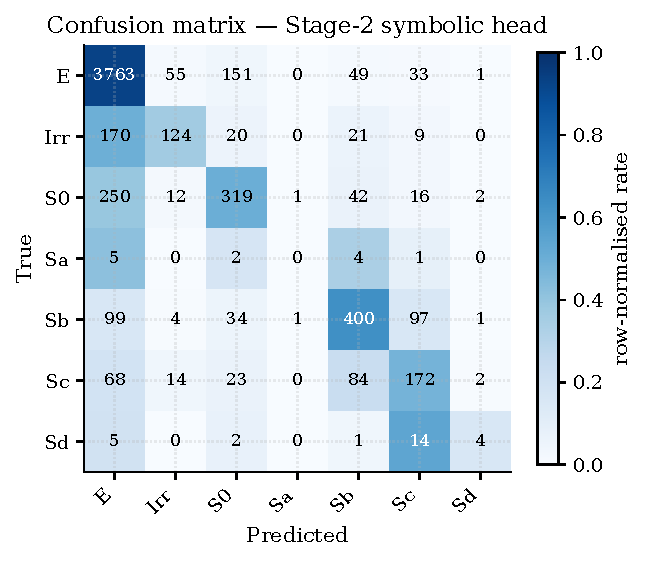
\includegraphics[width=\columnwidth]{figures/confusion.pdf}
\caption{Row-normalised confusion matrix for the symbolic head on the
validation split ($n=6075$). Cell annotations give raw counts. Misclassification
concentrates between adjacent Hubble types (Sb--Sc, E--S0), consistent with the
ordering of the morphological sequence; the Sa row is effectively empty at
$n=12$.}
\label{fig:confusion}
\end{figure}

\begin{figure}[htbp]
\centering
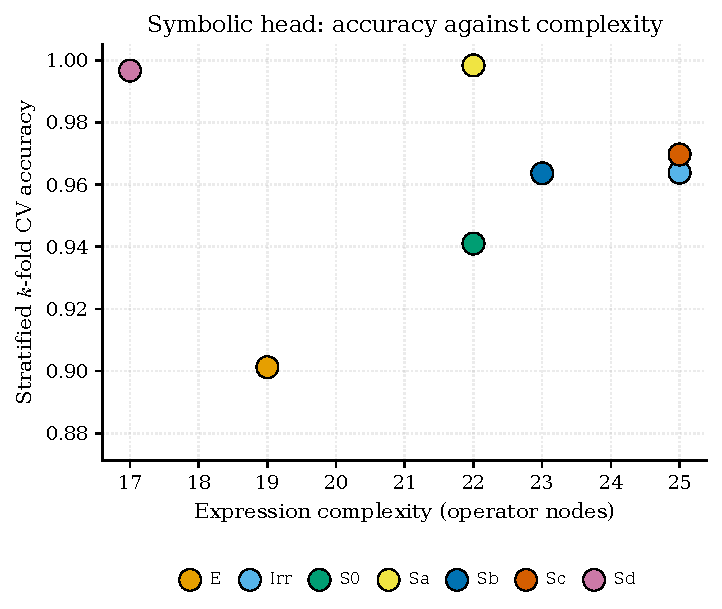
\includegraphics[width=\columnwidth]{figures/pareto.pdf}
\caption{Accuracy--complexity Pareto front per class. Markers indicate the
cross-validation-selected expression adopted for each class. The selected
rules occupy 17--25 nodes; expressions beyond this budget gained no
cross-validated accuracy.}
\label{fig:pareto}
\end{figure}

\subsection{Comparison against baselines}
\label{sec:baselines}

Table~\ref{tab:baselines} compares the symbolic head against three
alternatives trained on identical splits: a dense linear CBM head over the
same predicted concepts, gradient-boosted trees over the same concepts, and an
end-to-end ConvNeXt classifier with no bottleneck.

The unconstrained network is the most accurate model. It reaches accuracy
$0.802$ and $\kappa = 0.601$, ahead of the symbolic head by $0.015$ and
$0.030$ respectively. We report this plainly: passing predictions through a
seventeen-concept bottleneck and then through an analytic rule costs
approximately three points of $\kappa$ on this sample. Interpretability is not
free here, and any claim that it is would not survive the comparison.

The three concept-based models---symbolic, dense linear, boosted trees---are
mutually indistinguishable, spanning $0.001$ in accuracy and $0.002$ in
$\kappa$. The bottleneck, not the choice of head, is what separates them from
the network. This localises the cost: it is the restriction to seventeen named
concepts that gives up the three points, not the decision to express the final
classifier symbolically rather than densely. A practitioner who wants the
concept layer for auditability therefore pays once, and can then choose the
symbolic head at no further accuracy cost but with a large gain in legibility.

Macro-$F_1$ orders the models differently from accuracy and $\kappa$. The
symbolic head attains $0.462$ against the network's $0.448$, and the three
concept-based models all exceed the network on this metric. Accuracy and
$\kappa$ are dominated by the elliptical class, which supplies two thirds of
the sample; macro-$F_1$ weights all seven classes equally and therefore
reflects performance on the rare morphologies. The gap is small---$0.014$,
with Sa and Sd contributing at $n=12$ and $n=26$---and we do not claim it as a
significant advantage. We note only that the accuracy ranking and the
class-balanced ranking disagree, and that a reader interested in rare
morphologies should not select a model on accuracy alone.

The interpretability cost column makes the remaining trade explicit. The
symbolic head carries 153 operator nodes and is printed in full in
Table~\ref{tab:rules}; the network carries $1.5\times10^{7}$ trainable
parameters and cannot be printed at all. Three points of $\kappa$ is the price
of that difference on this dataset.

\begin{table}[htbp]
\centering
\caption{Baseline comparison on the validation split ($n=6075$), identical
splits and metrics throughout. Interpretability cost is measured in the
natural unit of each model class: operator nodes (symbolic), non-zero
coefficients (linear), retained features (boosted trees), trainable
parameters (network). All models are evaluated at their best validation
checkpoint. The unconstrained network leads on accuracy and $\kappa$; the
concept-based models lead on macro-$F_1$, which weights the rare classes
equally.}
\label{tab:baselines}
\small
\setlength{\tabcolsep}{5pt}
\begin{tabular}{lcccr}
\toprule
Model & Acc. & $F_1$ & \kappastat & Cost \\
\midrule
Symbolic CBM (this work) & 0.787 & \textbf{0.462} & 0.571 & $1.5\times10^{2}$ \\
Dense linear CBM         & 0.787 & 0.457 & 0.572 & $2.7\times10^{2}$ \\
XGBoost on concepts      & 0.786 & 0.450 & 0.570 & $3.9\times10^{1}$ \\
End-to-end ConvNeXt      & \textbf{0.802} & 0.448 & \textbf{0.601} & $1.5\times10^{7}$ \\
\bottomrule
\end{tabular}
\\[2pt]
\parbox{\columnwidth}{\footnotesize $F_1$ is macro-averaged. Interpretability:
the first two rows are intrinsically interpretable, XGBoost requires post-hoc
attribution, and the network is a black box. The concept bottleneck costs
$0.030$ in $\kappa$ relative to the unconstrained network; the choice of
symbolic versus dense head costs nothing further.}
\end{table}

\subsection{Do interpretable models agree with each other?}
\label{sec:agreement}

A concept-importance ranking is only useful if it is stable across reasonable
modelling choices. We compare the symbolic head's concept usage---each concept
weighted by the cross-validated accuracy of the rules invoking it---against the
linear head's coefficient magnitudes and against gradient-boosted-tree feature
importances, over the twenty concepts shared by all three.

Agreement is moderate: Spearman $\rho = 0.51$ (Pearson $0.60$) against the
linear head, and $\rho = 0.42$ (Pearson $0.67$) against boosted trees
(Fig.~\ref{fig:fidelity}). Three models trained on identical inputs, all
reaching the same accuracy, therefore rank the physical drivers of morphology
only partially consistently. This bounds how strongly any single model's
concept ranking should be read as a physical statement, and it argues for
reporting concept importance from an intrinsically interpretable model whose
ranking is the decision rule rather than a summary of one.

\begin{figure}[htbp]
\centering
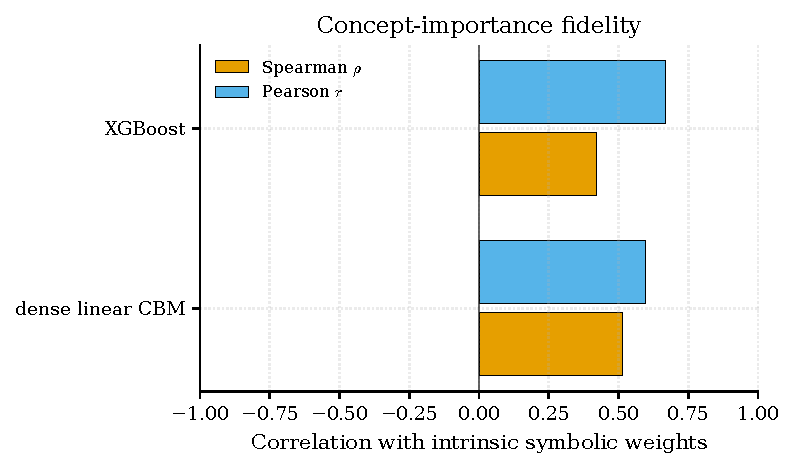
\includegraphics[width=\columnwidth]{figures/concept_fidelity.pdf}
\caption{Rank and linear correlation between the symbolic head's intrinsic
concept usage and the concept importances assigned by the dense linear head
and by gradient-boosted trees, over the twenty shared concepts. Agreement is
moderate, not high.}
\label{fig:fidelity}
\end{figure}

\subsection{Calibration: marginal validity, conditional failure}
\label{sec:calibration}

At $\alpha = 0.10$ the conformal wrapper attains $88.9\%$ empirical coverage
on the test split against a $90\%$ target, a deviation of $-0.011$, well
inside the finite-sample tolerance of $0.038$. Mean prediction-set size is
$1.46$ of seven classes and $66\%$ of test objects receive a singleton set.
Equation~\eqref{eq:coverage} is satisfied.

The sets also support a selective-prediction workflow.
Figure~\ref{fig:selective} plots accuracy on the retained sample against the
fraction abstained, under two acceptance rules: ranking by softmax confidence,
and accepting only when the conformal set contains fewer than $k$ classes.
Retained accuracy rises from $0.776$ on the full test split to $0.868$ at a
quarter deferred and $0.926$ at half, after which it is flat. A user willing
to send ambiguous objects to visual inspection can therefore trade
completeness for purity in a quantified way, and the plateau beyond $50\%$
abstention indicates that the residual errors are not ones the model's own
confidence can identify.

Table~\ref{tab:coverage} shows what that guarantee conceals. Coverage
conditional on true class ranges from $0.982$ for ellipticals to $0.083$ for
Sa. Irregulars are covered $45\%$ of the time and Sd $46\%$, against a nominal
$90\%$. The marginal guarantee is met because ellipticals constitute two
thirds of the sample and are over-covered; every rare class is far below
nominal.

This behaviour is expected---marginal conformal prediction makes no
conditional promise---but its magnitude here has direct scientific
consequence. A researcher selecting irregular or Sd candidates from this
catalogue and trusting the nominal $90\%$ would be operating at roughly half
that coverage, and for Sa the prediction sets are essentially uninformative.
Reporting only marginal coverage in a morphology context is therefore
misleading, and we recommend that per-class coverage accompany any conformal
result on imbalanced astronomical samples. Class-conditional conformal
methods~\citep{ding2023classcond} address this directly and are the natural
next step.

\begin{table}[htbp]
\centering
\caption{Conformal coverage by true class on the test split at nominal
$1-\alpha = 0.90$. Marginal coverage is $0.889$. The guarantee is satisfied
marginally while failing badly for every class other than E.}
\label{tab:coverage}
\begin{tabular}{lrrr}
\toprule
Class & $n$ & Coverage & Mean $|C(x)|$ \\
\midrule
E   & 4052 & 0.982 & 1.28 \\
Sb  &  636 & 0.863 & 1.69 \\
S0  &  643 & 0.728 & 1.76 \\
Sc  &  362 & 0.657 & 2.16 \\
Sd  &   26 & 0.462 & 2.31 \\
Irr &  344 & 0.451 & 1.73 \\
Sa  &   12 & 0.083 & 2.08 \\
\midrule
\textbf{Marginal} & 6075 & \textbf{0.889} & \textbf{1.46} \\
\bottomrule
\end{tabular}
\end{table}

\begin{figure}[htbp]
\centering
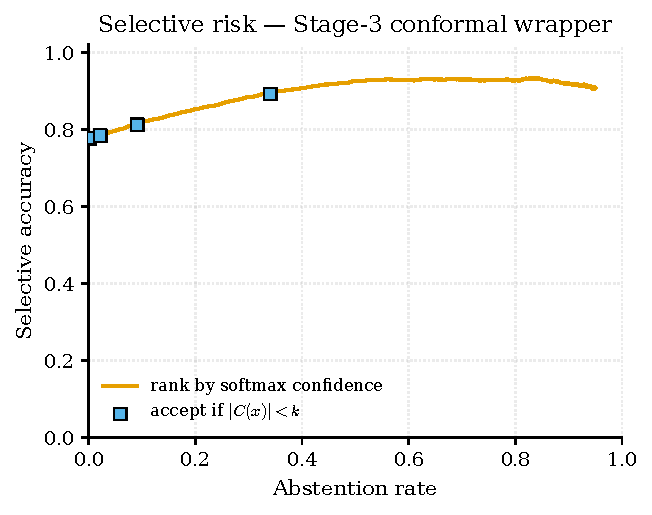
\includegraphics[width=\columnwidth]{figures/selective_risk.pdf}
\caption{Selective accuracy against abstention rate. Ranking by softmax
confidence (curve) and by conformal set size (markers) both concentrate
correct predictions at low abstention, so a downstream user can trade
completeness for purity in a controlled way.}
\label{fig:selective}
\end{figure}

\subsection{Cross-survey transfer}
\label{sec:robustness}

We apply the frozen Stage-1$\rightarrow$2$\rightarrow$3 pipeline to
$161\,395$ Euclid Q1 galaxies and, separately, refit the symbolic head on a
stratified Euclid subsample to measure rule stability
(Table~\ref{tab:robustness}, Fig.~\ref{fig:shift}).

Classification transfers. Accuracy rises by $0.052$ and $\kappa$ by $0.170$
relative to the DECaLS reference. This is not a majority-class artefact:
Euclid's label distribution is \emph{less} elliptical-dominated ($57.2\%$
versus $66.8\%$), which should if anything depress a prior-driven classifier.
We caution that the comparison is not controlled---the two surveys differ in
depth, resolution, passband and volunteer campaign, and the Euclid labels come
from a different vote-fraction distribution---so we report the transfer as an
observation, not as evidence that Euclid morphology is intrinsically easier.

Calibration degrades. Expected calibration error rises by $0.083$: the
pipeline becomes more accurate and simultaneously less able to signal when it
should not be trusted. Confidence ranking is the first casualty of domain
shift, before accuracy.

Explanations do not transfer. A symbolic refit on Euclid recovers a mean
per-class concept-usage Jaccard of $0.420$ and a top-five concept overlap of
$0.429$. Fewer than half the concepts that the reference rules rely on
reappear when the same procedure is run on the shifted survey. The functional
form of ``how to recognise a spiral'' is instrument-dependent even where the
resulting labels are not.

This is the paper's central methodological point. An accuracy-only robustness
audit of this pipeline would report improvement under shift and certify it as
transferable. Two additional measurements---conditional coverage and rule
stability---show that the uncertainty quantification and the explanation have
both silently changed. Accuracy transfer, calibration transfer and
interpretation transfer are three separate properties, and only the first is
routinely reported.

\begin{table}[htbp]
\centering
\caption{DECaLS $\rightarrow$ Euclid Q1 transfer. $\Delta$ denotes shifted
minus reference. Jaccard indices are defined in
Equation~\eqref{eq:jaccard}; $1$ denotes identical concept usage.}
\label{tab:robustness}
\begin{tabular}{lr}
\toprule
Quantity & Value \\
\midrule
$n$ reference / shifted & 6075 / 161395 \\
$\Delta$ accuracy & $+0.052$ \\
$\Delta$ macro-$F_1$ & $+0.204$ \\
$\Delta\,\kappastat$ & $+0.170$ \\
$\Delta$ ECE & $+0.083$ \\
$\Delta$ conformal coverage & $+0.074$ \\
\midrule
Rule stability, mean per-class $J$ & $0.420$ \\
Rule stability, top-5 concept $J$ & $0.429$ \\
\bottomrule
\end{tabular}
\end{table}

\begin{figure}[htbp]
\centering
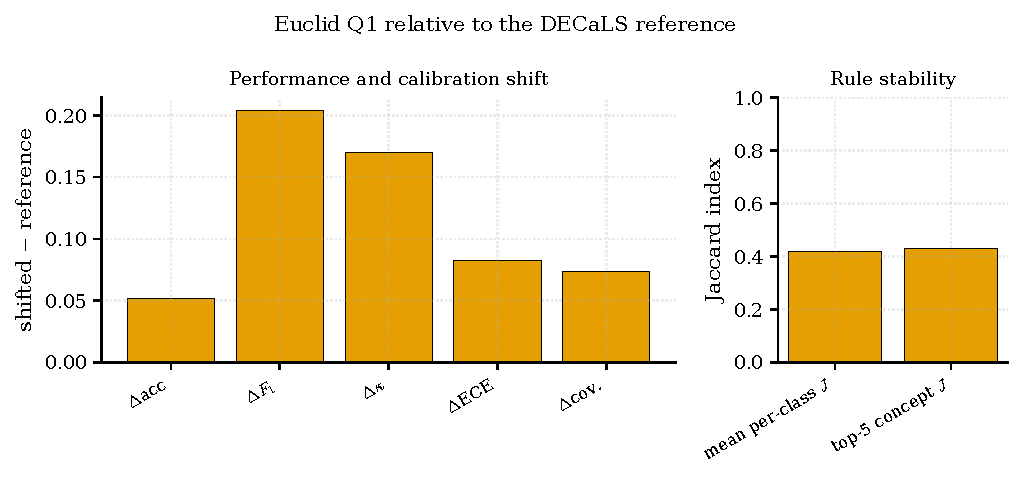
\includegraphics[width=\columnwidth]{figures/robustness_shift.pdf}
\caption{Cross-survey transfer from DECaLS to Euclid Q1. Classification
metrics improve while calibration error rises and rule-stability indices sit
below $0.45$, separating accuracy transfer from interpretation transfer.}
\label{fig:shift}
\end{figure}

%=======================================================================
\section{Discussion}
\label{sec:discussion}

\subsection{What the rule table buys}

The deployed classifier is Table~\ref{tab:rules}. A referee can read it, check
that the elliptical rule keys on smoothness and the absence of merger
signatures, verify that spiral subtypes separate on winding and bulge size,
and identify exactly which concept would have to change to flip a
classification. That audit is available for a black-box network only through a
surrogate whose faithfulness is itself in question~\citep{rudin2019}, and
Section~\ref{sec:agreement} shows that surrogate rankings disagree
substantially with the intrinsic rule even when accuracy matches.

The recovered rules reproduce the branching order of the Galaxy Zoo decision
tree without being told it. That is a consistency check rather than a
discovery, but it is the kind of check that an uninterpretable model cannot
offer.

What that audit costs is now quantified rather than asserted: $0.030$ in
$\kappa$ against an unconstrained network (Section~\ref{sec:baselines}).
Because the three concept-based models agree to within $0.002$, the price is
attributable to the concept layer and not to the symbolic form of the head.
This matters for anyone adopting the architecture. Having accepted a concept
bottleneck for auditability, one may take the symbolic head---and with it a
classifier small enough to print---without giving up anything further. The
design decision worth deliberating is whether to impose the bottleneck at all;
the choice of head, once inside it, is close to free.

\subsection{What conditional coverage means for rare-object science}

The morphologies of greatest astrophysical interest are frequently the rarest:
mergers, disturbed systems, edge-on discs with dust lanes. Table~\ref{tab:coverage}
shows these are exactly the classes for which marginal conformal guarantees
fail hardest. Any selection function built on nominal coverage will be
optimistic by a factor of two for irregulars in this sample. We regard this as
the most practically consequential result here: the fix is
class-conditional conformal calibration, which trades set size for
per-class validity, and we recommend it as the default in imbalanced
astronomical settings rather than the marginal variant.

\subsection{Interpretation transfer as an evaluation target}

Domain-shift studies in astronomy report accuracy degradation and remedy it by
retraining or domain adaptation. Section~\ref{sec:robustness} shows that the
explanation can change even when accuracy does not, which no accuracy-based
diagnostic detects. If interpretable models are to be deployed across the
survey landscape of the next decade---Euclid, LSST, Roman---then rule
stability under instrument change is a property that must be measured, not
assumed. Equation~\eqref{eq:jaccard} is a deliberately simple instrument for
this; more refined measures of functional-form equivalence are an open
problem.

The physical driver of the instability is plausibly the resolution and
passband dependence of the concept layer itself~\citep{ferrari2015}: if
smoothness and asymmetry mean different things at $0.262''$ and $0.1''$
sampling, rules built on them cannot be expected to survive. Disentangling
concept-level from rule-level instability requires matched-resolution
experiments we have not performed.

%=======================================================================
\section{Limitations}
\label{sec:limitations}

We state the constraints on these results explicitly.

\emph{Class imbalance dominates the aggregate metrics.} With 49 Sa and 104 Sd
training examples, no conclusion about these classes is supported by these
data. Macro-$F_1$ of $0.462$ against accuracy of $0.787$ is a direct
consequence, and the high one-vs-rest CV accuracies in
Table~\ref{tab:rules} for rare classes reflect class prior, not discrimination.

\emph{Interpretability costs accuracy here.} The unconstrained network leads
the symbolic head by $0.030$ in $\kappa$ (Table~\ref{tab:baselines}). We do not
claim that symbolic regression is the better classifier. The claim is narrower:
the concept bottleneck carries a measurable and modest price, the symbolic form
adds nothing to that price, and the resulting model is auditable. Whether three
points of $\kappa$ is worth paying is an application-dependent judgement we
leave to the reader.

\emph{Baseline training budget.} All models are evaluated at their best
validation checkpoint. The network overfits within a few epochs at this sample
size and its early-stopped optimum may not be its ceiling; a larger training
set (Section~\ref{sec:data}) would likely favour it further, which would widen
rather than close the gap we report.

\emph{The concept vocabulary is closed.} Structural properties absent from
both the Galaxy Zoo tree and \textsc{statmorph} cannot enter a rule, and
therefore cannot be diagnosed as a cause of transfer failure. Our inability to
attribute the Euclid rule instability to a specific instrumental cause follows
from this.

\emph{The cross-survey comparison is uncontrolled.} DECaLS and Euclid Q1
differ in depth, resolution, passband and volunteer campaign simultaneously.
The transfer numbers in Table~\ref{tab:robustness} describe what happens, not
why.

\emph{Two concepts fail.} Smoothness does not beat its trivial baseline and
asymmetry is marginal; rules invoking them inherit that weakness.

\emph{The symbolic refit is subsampled.} Euclid rule stability is computed on
a $3000$-object stratified subsample for tractability. The indices should be
reconfirmed at full survey scale.

\emph{Softmax scores are not probabilities.} Conformal coverage holds
regardless, but the ECE shift in Table~\ref{tab:robustness} should be read as
degraded confidence \emph{ranking}, not as miscalibration of a probabilistic
model.

\emph{One shifted survey.} The HST/JWST leg is pending data access; the
three-survey claim is currently a two-survey result.

%=======================================================================
\section{Conclusions}
\label{sec:conclusions}

We built a Concept Bottleneck Model for galaxy morphology in which a symbolic
rule set of 153 operator nodes performs the final classification, wrapped in
split-conformal prediction. On $40\,498$ Galaxy Zoo Evo galaxies:

\begin{enumerate}
\item The concept bottleneck costs $0.030$ in $\kappa$ relative to an
unconstrained ConvNeXt, while the symbolic head, a dense linear head and
gradient-boosted trees over the same concepts agree to within $0.002$. The
price is paid for the bottleneck, not for the symbolic form, and buys a
classifier of 153 operator nodes in place of $1.5\times10^{7}$ parameters. On
macro-$F_1$ the ordering reverses and every concept-based model exceeds the
network.
\item Fifteen of seventeen concepts are recovered above trivial baselines, and
the discovered rules reproduce the branching structure of the Galaxy Zoo
decision tree without supervision on that structure.
\item Marginal conformal coverage is exact ($0.889$ against $0.90$) while
conditional coverage spans $0.98$ to $0.08$ across classes. Marginal
guarantees are inadequate for rare-morphology science, and per-class coverage
should be reported as standard.
\item Under DECaLS $\rightarrow$ Euclid transfer, accuracy is preserved while
calibration degrades and symbolic refits recover under half the reference
concept usage. Accuracy transfer does not imply interpretation transfer.
\end{enumerate}

The third and fourth findings generalise beyond this model. Any interpretable
classifier deployed across surveys inherits both failure modes, and neither is
visible to the accuracy-based diagnostics currently reported. We release the
benchmark so that concept fidelity, conditional coverage and rule stability
can be measured for any morphology pipeline.

%=======================================================================
\section*{Data and code availability}
\label{sec:availability}

% NOTE: this repository is currently PRIVATE. It must be made public (or a
% Zenodo DOI minted from it) before submission, or this statement is false.
All code, configurations, random seeds and derived results are available at
\url{https://github.com/ramc77/GalaxyCBM-SR}. The pipeline reproduces from a
single \code{make all}; every number quoted in this paper is written to
\code{results/metrics.json} by the evaluation stage and verified against a
manifest of paper claims at build time. Galaxy Zoo Evo, Euclid Q1 and
Galaxy Zoo JWST data are public
\citep{walmsley2025gzevo,euclid2025morphology}.

%=======================================================================
% Elsevier requires both statements below for Astronomy and Computing.
\section*{CRediT authorship contribution statement}

\textbf{Ram Chand:} Conceptualization, Methodology, Software, Validation,
Formal analysis, Investigation, Data curation, Writing --- original draft,
Writing --- review and editing, Visualization.

\section*{Declaration of competing interest}

The author declares that he has no known competing financial interests or
personal relationships that could have appeared to influence the work reported
in this paper.

\section*{Acknowledgments}
We thank the Galaxy Zoo volunteers, whose classifications constitute the
concept layer of this model, and the Galaxy Zoo and Euclid teams for releasing
the morphology catalogues used here. Computations were performed in the
computing laboratory of the Department of Natural Sciences, The Begum Nusrat
Bhutto Women University, Sukkur.

This work uses data from Galaxy Zoo Evo~\citep{walmsley2025gzevo}, Galaxy Zoo
DECaLS~\citep{walmsley2022}, Galaxy Zoo DESI~\citep{walmsley2023desi} and the
Euclid Q1 visual morphology catalogue~\citep{euclid2025morphology}. The
analysis relies on \textsc{Zoobot}~\citep{walmsley2023zoobot},
\textsc{statmorph}~\citep{rodriguez2019}, PySR~\citep{cranmer2023} and
MAPIE~\citep{taquet2022}.


%=======================================================================
% All entries below verified against arXiv / publisher records.
% Classic astronomy references (Hubble 1926; Conselice 2003, 2014; Lotz 2004;
% Ferrari 2015; Dieleman 2015; Dominguez Sanchez 2018) should still be
% re-checked against ADS at submission time for page/volume accuracy.
\clearpage
\begin{thebibliography}{99}

\bibitem[Angelopoulos \& Bates(2023)]{angelopoulos2023}
Angelopoulos, A.~N., \& Bates, S. 2023, \emph{A Gentle Introduction to
Conformal Prediction and Distribution-Free Uncertainty Quantification},
Foundations and Trends in Machine Learning, 16, 494; arXiv:2107.07511

\bibitem[Conselice(2003)]{conselice2003}
Conselice, C.~J. 2003, \emph{The Relationship between Stellar Light
Distributions of Galaxies and Their Formation Histories}, \apjs, 147, 1

\bibitem[Conselice(2014)]{conselice2014}
Conselice, C.~J. 2014, \emph{The Evolution of Galaxy Structure over Cosmic
Time}, \araa, 52, 291

\bibitem[Cranmer(2023)]{cranmer2023}
Cranmer, M. 2023, \emph{Interpretable Machine Learning for Science with PySR
and SymbolicRegression.jl}, arXiv:2305.01582

\bibitem[Dieleman et al.(2015)]{dieleman2015}
Dieleman, S., Willett, K.~W., \& Dambre, J. 2015,
\emph{Rotation-Invariant Convolutional Neural Networks for Galaxy Morphology
Prediction}, \mnras, 450, 1441

\bibitem[Ding et al.(2023)]{ding2023classcond}
Ding, T., Angelopoulos, A.~N., Bates, S., Jordan, M.~I., \& Tibshirani, R.~J.
2023, \emph{Class-Conditional Conformal Prediction with Many Classes}, in
Advances in Neural Information Processing Systems 36 (NeurIPS 2023);
arXiv:2306.09335

\bibitem[Domínguez Sánchez et al.(2018)]{dominguez2018}
Domínguez Sánchez, H., Huertas-Company, M., Bernardi, M., Tuccillo, D., \&
Fischer, J.~L. 2018, \emph{Improving Galaxy Morphologies for SDSS with Deep
Learning}, \mnras, 476, 3661

\bibitem[Euclid Collaboration: Walmsley et al.(2026)]{euclid2025morphology}
Euclid Collaboration: Walmsley, M., Huertas-Company, M., Quilley, L., et al.
2026, \emph{Euclid Quick Data Release (Q1) --- IX. First Visual Morphology
Catalogue}, \aap; arXiv:2503.15310

\bibitem[Ferrari et al.(2015)]{ferrari2015}
Ferrari, F., de Carvalho, R.~R., \& Trevisan, M. 2015,
\emph{Morfometryka --- A New Way of Establishing Morphological Classification
of Galaxies}, \apj, 814, 55

\bibitem[Hubble(1926)]{hubble1926}
Hubble, E.~P. 1926, \emph{Extragalactic Nebulae}, \apj, 64, 321

\bibitem[Koh et al.(2020)]{koh2020}
Koh, P.~W., Nguyen, T., Tang, Y.~S., Mussmann, S., Pierson, E., Kim, B., \&
Liang, P. 2020, \emph{Concept Bottleneck Models}, in Proc.\ 37th International
Conference on Machine Learning (ICML), PMLR 119, 5338; arXiv:2007.04612

\bibitem[Liu et al.(2022)]{liu2022convnext}
Liu, Z., Mao, H., Wu, C.-Y., Feichtenhofer, C., Darrell, T., \& Xie, S. 2022,
\emph{A ConvNet for the 2020s}, in Proc.\ IEEE/CVF Conference on Computer
Vision and Pattern Recognition (CVPR), 11976; arXiv:2201.03545

\bibitem[Lotz et al.(2004)]{lotz2004}
Lotz, J.~M., Primack, J., \& Madau, P. 2004, \emph{A New Nonparametric
Approach to Galaxy Morphological Classification}, \aj, 128, 163

\bibitem[Lundberg \& Lee(2017)]{lundberg2017}
Lundberg, S.~M., \& Lee, S.-I. 2017, \emph{A Unified Approach to Interpreting
Model Predictions}, in Advances in Neural Information Processing Systems 30
(NIPS 2017), 4765; arXiv:1705.07874

\bibitem[Oikarinen et al.(2023)]{oikarinen2023}
Oikarinen, T., Das, S., Nguyen, L.~M., \& Weng, T.-W. 2023,
\emph{Label-Free Concept Bottleneck Models}, in Proc.\ 11th International
Conference on Learning Representations (ICLR); arXiv:2304.06129

\bibitem[Rodriguez-Gomez et al.(2019)]{rodriguez2019}
Rodriguez-Gomez, V., Snyder, G.~F., Lotz, J.~M., et al. 2019,
\emph{The Optical Morphologies of Galaxies in the IllustrisTNG Simulation: A
Comparison to Pan-STARRS Observations}, \mnras, 483, 4140

\bibitem[Rudin(2019)]{rudin2019}
Rudin, C. 2019, \emph{Stop Explaining Black Box Machine Learning Models for
High Stakes Decisions and Use Interpretable Models Instead}, Nature Machine
Intelligence, 1, 206; arXiv:1811.10154

\bibitem[Smilkov et al.(2017)]{smilkov2017}
Smilkov, D., Thorat, N., Kim, B., Viégas, F., \& Wattenberg, M. 2017,
\emph{SmoothGrad: Removing Noise by Adding Noise}, arXiv:1706.03825

\bibitem[Taquet et al.(2022)]{taquet2022}
Taquet, V., Blot, V., Morzadec, T., Lacombe, L., \& Brunel, N. 2022,
\emph{MAPIE: An Open-Source Library for Distribution-Free Uncertainty
Quantification}, arXiv:2207.12274

\bibitem[Vovk et al.(2005)]{vovk2005}
Vovk, V., Gammerman, A., \& Shafer, G. 2005, \emph{Algorithmic Learning in a
Random World} (New York: Springer)

\bibitem[Walmsley et al.(2022)]{walmsley2022}
Walmsley, M., Lintott, C., Géron, T., et al. 2022, \emph{Galaxy Zoo DECaLS:
Detailed Visual Morphology Measurements from Volunteers and Deep Learning for
314\,000 Galaxies}, \mnras, 509, 3966

\bibitem[Walmsley et al.(2023a)]{walmsley2023zoobot}
Walmsley, M., Allen, C., Aussel, B., et al. 2023a, \emph{Zoobot: Adaptable
Deep Learning Models for Galaxy Morphology}, Journal of Open Source Software,
8(85), 5312

\bibitem[Walmsley et al.(2023b)]{walmsley2023desi}
Walmsley, M., Géron, T., Kruk, S., et al. 2023b, \emph{Galaxy Zoo DESI:
Detailed Morphology Measurements for 8.7M Galaxies in the DESI Legacy Imaging
Surveys}, \mnras, 526, 4768; arXiv:2309.11425

\bibitem[Walmsley et al.(2024)]{walmsley2024scaling}
Walmsley, M., Bowles, M., Scaife, A.~M.~M., et al. 2024, \emph{Scaling Laws
for Galaxy Images}, arXiv:2404.02973

\bibitem[Walmsley et al.(2025)]{walmsley2025gzevo}
Walmsley, M., et al. 2025, \emph{Galaxy Zoo Evo: 1 Million Human-Annotated
Images of Galaxies}, arXiv:2512.23691

\bibitem[Yuksekgonul et al.(2023)]{yuksekgonul2023}
Yuksekgonul, M., Wang, M., \& Zou, J. 2023, \emph{Post-hoc Concept Bottleneck
Models}, in Proc.\ 11th International Conference on Learning Representations
(ICLR), Spotlight; arXiv:2205.15480

\bibitem[Deshpande \& Desai(2026)]{deshpande2026}
Deshpande, R., \& Desai, S. 2026, \emph{Comparison of Symbolic Regression
Algorithms in Star/Galaxy/Quasar Separation}, arXiv:2602.24022

\bibitem[Llorella \& Cebrian(2025)]{llorella2025}
Llorella, F.~R., \& Cebrian, J.~A. 2025, \emph{Exploring Symbolic Regression
and Genetic Algorithms for Astronomical Object Classification}, The Open
Journal of Astrophysics, 8; \doi{10.33232/001c.132333}; arXiv:2503.09220

\end{thebibliography}

\end{document}
